\section{Siglo XXI}

\begin{figure}[tb]
  \centering
  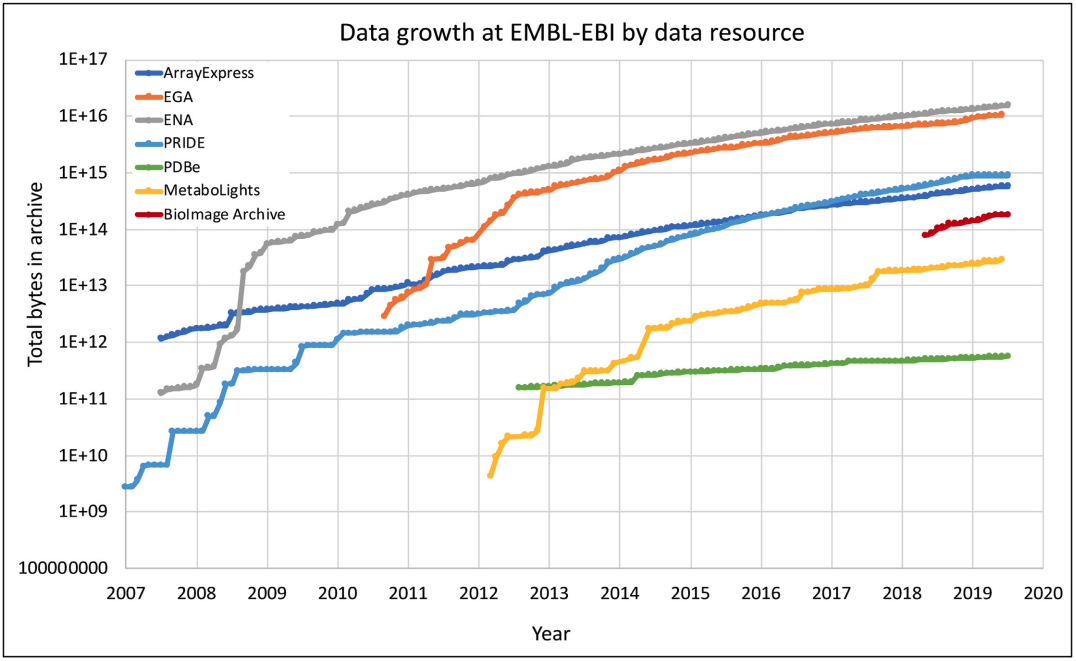
\includegraphics[width=0.9\columnwidth]{images/Dat_trend.png}
  \caption{
      (\textit{Figura en inglés})
      Crecimiento exponencial de los datos manejados por el Instituto Europeo de Bioinformática (EMBL-EBI).
      Note que un Terabyte son $10^{12}$ bytes.
      En la gráfica se muestra la evolución de diferentes bases de datos, desde genómicas hasta imágenes de microscopía.
      Para más detalles ir a la Fuente \cite{cookEuropeanBioinformaticsInstitute2020}
  }
  \label{fig:Dat_trend}
\end{figure}

En las últimas dos décadas la Biología se ha posicionado como una de las ciencias que genera mayor cantidad de datos.
Por ejemplo, en el 2015, la cantidad de genomas humanos secuenciados se duplicaba cada 7 meses.
O sea, si a comienzos de los 2000 tras una década de trabajo se publicaba el primer genoma de humano, veinte años después se acumulan más de un millón.
¿Y es eso mucho?
Como referencia tomen que, en 2015, \textit{youtube} generó entre 1-2 exabytes (millones de terabytes) de nuevo contenido, mientras que se estima que la genómica como campo pudo generar hasta 40 \cite{stephensBigDataAstronomical2015}.
Esta tendencia no es única para la genómica.
Cada elemento de interés biológico está siendo estudiado y recopilado en enormes bases de datos.
¡Hay curvas de crecimiento exponencial por todos lados! (figura \ref{fig:Dat_trend}).

A pesar de esto, aunque es un gran reto, el almacenamiento no es el mayor de los problemas a enfrentar en la actualidad.
Más agudo aún es el de extraer de los datos la información relevante.
Por ejemplo, si reevaluamos el alineamiento de secuencias en el contexto contemporáneo veremos la magnitud del reto.
El alineamiento de un genoma completo de humano con otro de ratón, usando los últimos algoritmos, toma alrededor de 100 horas ($\sim$ 4 días) en un CPU moderno.
Ahora, si escalamos este análisis para todos los genomas de las más de 2.5 millones de especies que se espera tener secuenciadas para el 2025, se necesitaría toda la capacidad actual de cómputo de la humanidad multiplicada por un millón \cite{stephensBigDataAstronomical2015}.
¿Pero acaso la humanidad no está aumentando su poder de cómputo exponencialmente? ¿No se puede simplemente esperar hasta que sea suficiente?
Pues no es tan simple, mientras que la evolución del poder de cómputo ha seguido la tendencia de duplicarse cada 2 años (llamada Ley de Moore), incluso aunque esta se mantenga, la generación de datos biológicos es simplemente mucho mayor (es duplicada en menos de un año) \cite{stephensBigDataAstronomical2015}.
A esto se le suma el hecho de que hay otras áreas de la actividad humana generando cantidades similares de datos, desde la Astrofísica hasta las redes sociales.
No todas las computadoras son para nosotros.

La discusión anterior ilustra sólo una parte del problema: el enorme volumen de datos dificulta incluso la aplicación de técnicas ya establecidas.
Pero otro igual de significativo es el de generar nuevas formas de análisis.
Por ejemplo, en la era pre-ómicas, las áreas de la Biología que intentaban construir modelos detallados de sistemas completos no atraían mucho interés.
Los sistemas vivos son simplemente muy complejos. 
Estos pueden comprender miles de componentes por cada célula, miles de tipos celulares por cada organismo y un sin número de especies diferentes por ecosistema.
Todo ello extremadamente interconectado y sometido a cambios constantes.
Sin los datos suficientes, la creación de modelos capaces de capturar tal complejidad estaba fuera del alcance de los investigadores.
Pero en los últimos años la situación es diferente, como se evidencia con la consolidación de la Biología de Sistemas \cite{likicSystemsBiologyNext2010a}.
Esta disciplina intenta explicar detalladamente la relación que enuncia el dogma central y sus consecuencias:
¿cómo el genoma determina función?
Este nuevo enfoque mueve el centro de estudio desde el \textit{elemento} a la \textit{red de elementos}.
O sea, se trata de explicar cómo una determinada función emerge de la interacción de las partes del sistema.
Lo cual es posible  solo si se tienen datos lo suficientemente completos para representar una parte significativa del mismo.

\begin{figure}[tb]
  \centering
  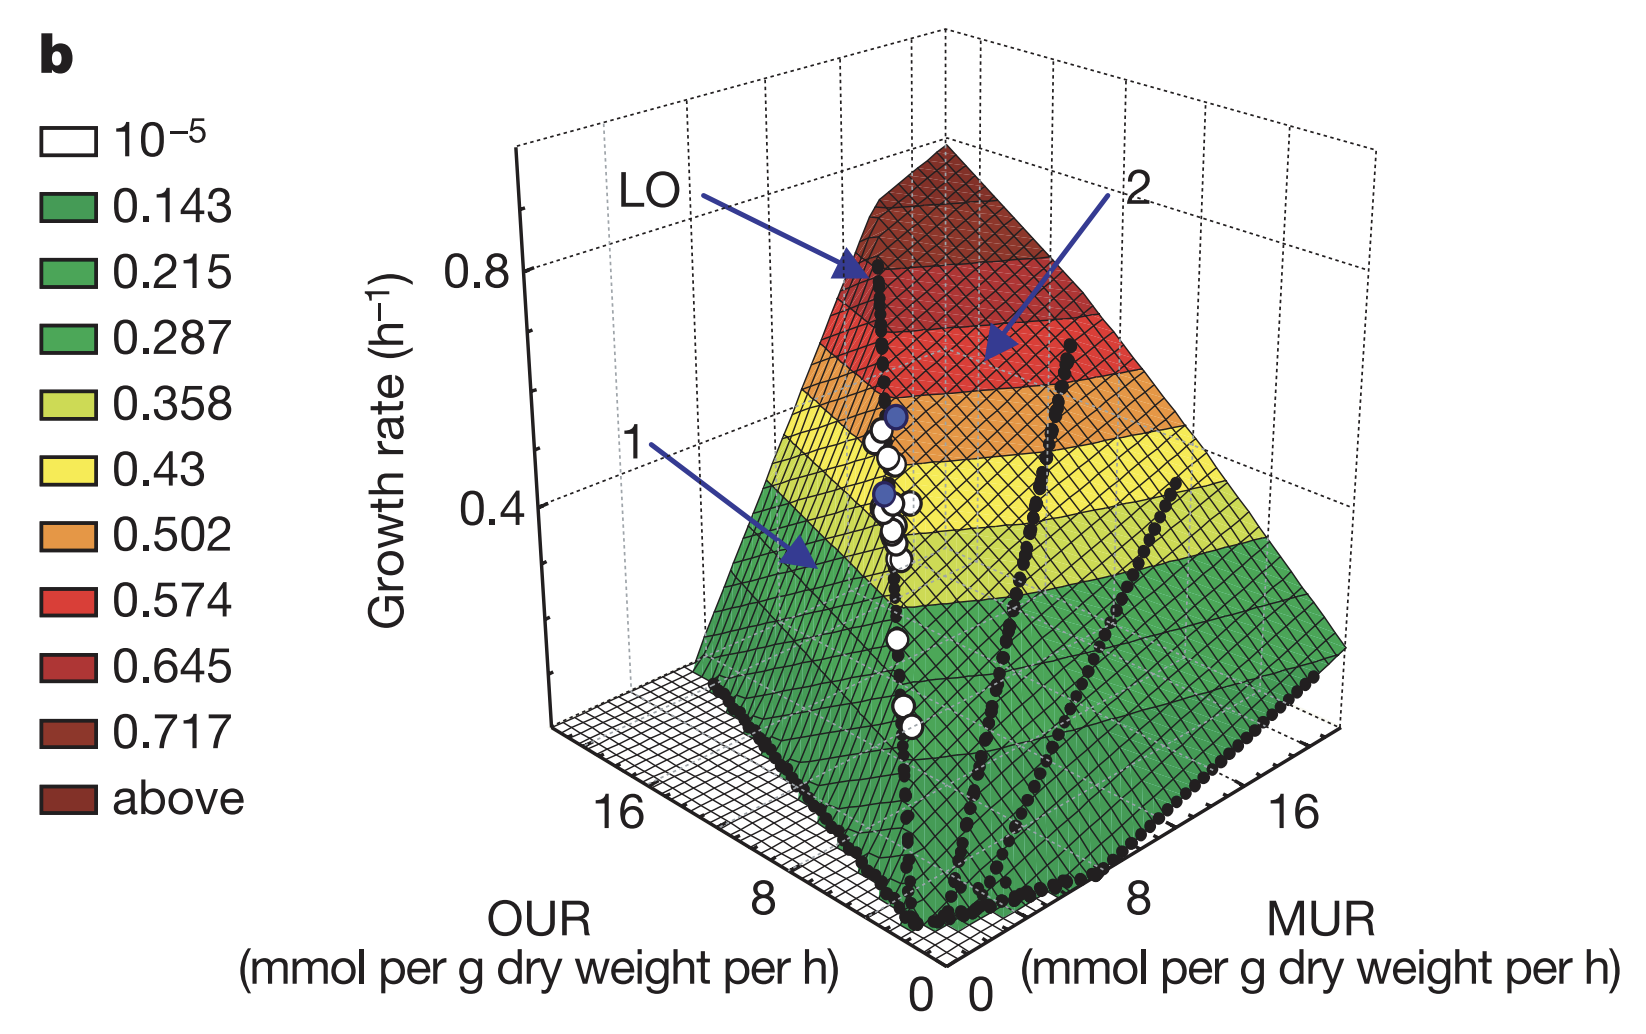
\includegraphics[width=0.9\columnwidth]{images/Ecoli_growth.png}
  \caption{
      (\textit{Figura en inglés})
      En la figura se muestra cómo dadas las disponibilidades de malato (MUR) y oxígeno (OUR), principales nutrientes limitantes en el cultivo, el crecimiento de la bacteria (círculos blancos y azules) sigue la tendencia esperada descrita por el modelo (puntos negros).
      Para más detalles ir a \cite{ibarraEscherichiaColiK122002}
  }
  \label{fig:Ecoli_growth}
\end{figure}

Por ejemplo, hoy se dispone de redes que comprenden todas las reacciones metabólicas que se han identificado en el genoma de $\textit{Escherichia coli}$.
Con estas redes se pueden construir modelos para simular el crecimiento de dicha bacteria en un medio dado.
A medida que más datos se le han ido incorporando a estos modelos, estos han ido mejorando su poder predictivo \cite{ibarraEscherichiaColiK122002}.
Además de las aplicaciones ingenieriles que se pueden derivar, la modelación también contribuye a generar conocimientos biológicos.
En los resultados mostrados en la figura \ref{fig:Ecoli_growth}, por ejemplo, los valores experimentales (círculos blancos y azules) se ubican en el máximo posible dada las restricciones que establece el modelo.
O sea, las bacterias están creciendo tanto como pueden dada la disponibilidad de nutrientes y su capacidad metabólica, lo cual pudiera ser referente de la presión adaptativa a la que se enfrentan típicamente en su ambiente natural.
En general, avances como este hacen que la Biología se mueva cada vez más de su enfoque experimental de ``prueba y error'' a otro mucho más teóricamente intenso.

Por otro lado, la disponibilidad de grandes cantidades de datos sin analizar no haya pasado inadvertida pora otras disciplinas.
Físicos, ingenieros, científicos de la Computación y muchos otros especialistas están tratando de modificar las técnicas y habilidades que emplean en sus campos para analizar los datos biológicos.
Un ejemplo reciente es el caso de \textit{DeepMind}, una subsidiaria de \textit{google}.
Anteriormente, en el año 2017, esta empresa de inteligencia artificial logró el hito de crear un programa para jugar \textit{Go} que pudo vencer al jugador humano con el primer puesto en el ranking de ese deporte.
Pero en el año 2020, \textit{DeepMind} volvió a ser noticia.
Esta vez fue por usar su enorme capacidad para atacar lo que es considerado uno de los problemas computacionales más grandes de la Biología: predecir la estructura 3D de las proteínas a partir de su secuencia lineal \cite{callawayItWillChange2020}.
En particular, \textit{DeepMind} sobrepasó a otros 100 equipos en un concurso bianual llamado $\textit{CAPS}$.
En este concurso alrededor de 100 secuencias de proteínas son publicadas.
Las estructuras 3D de estas proteínas son determinadas a partir de técnicas experimentales ya establecidas pero esta información no es pública hasta después del concurso.
Así, los equipos tienen dos años para proponer sus propias estructuras que luego son comparadas con las experimentales.
El uso masivo por parte de $\textit{DeepMind}$ de nuevas técnicas de $\textit{Machine Learning}$ les permitió obtener resultados revolucionarios en esta área (figura \ref{fig:Deep_Mind}) \cite{callawayItWillChange2020}.
 
\begin{figure}[tb]
  \centering
  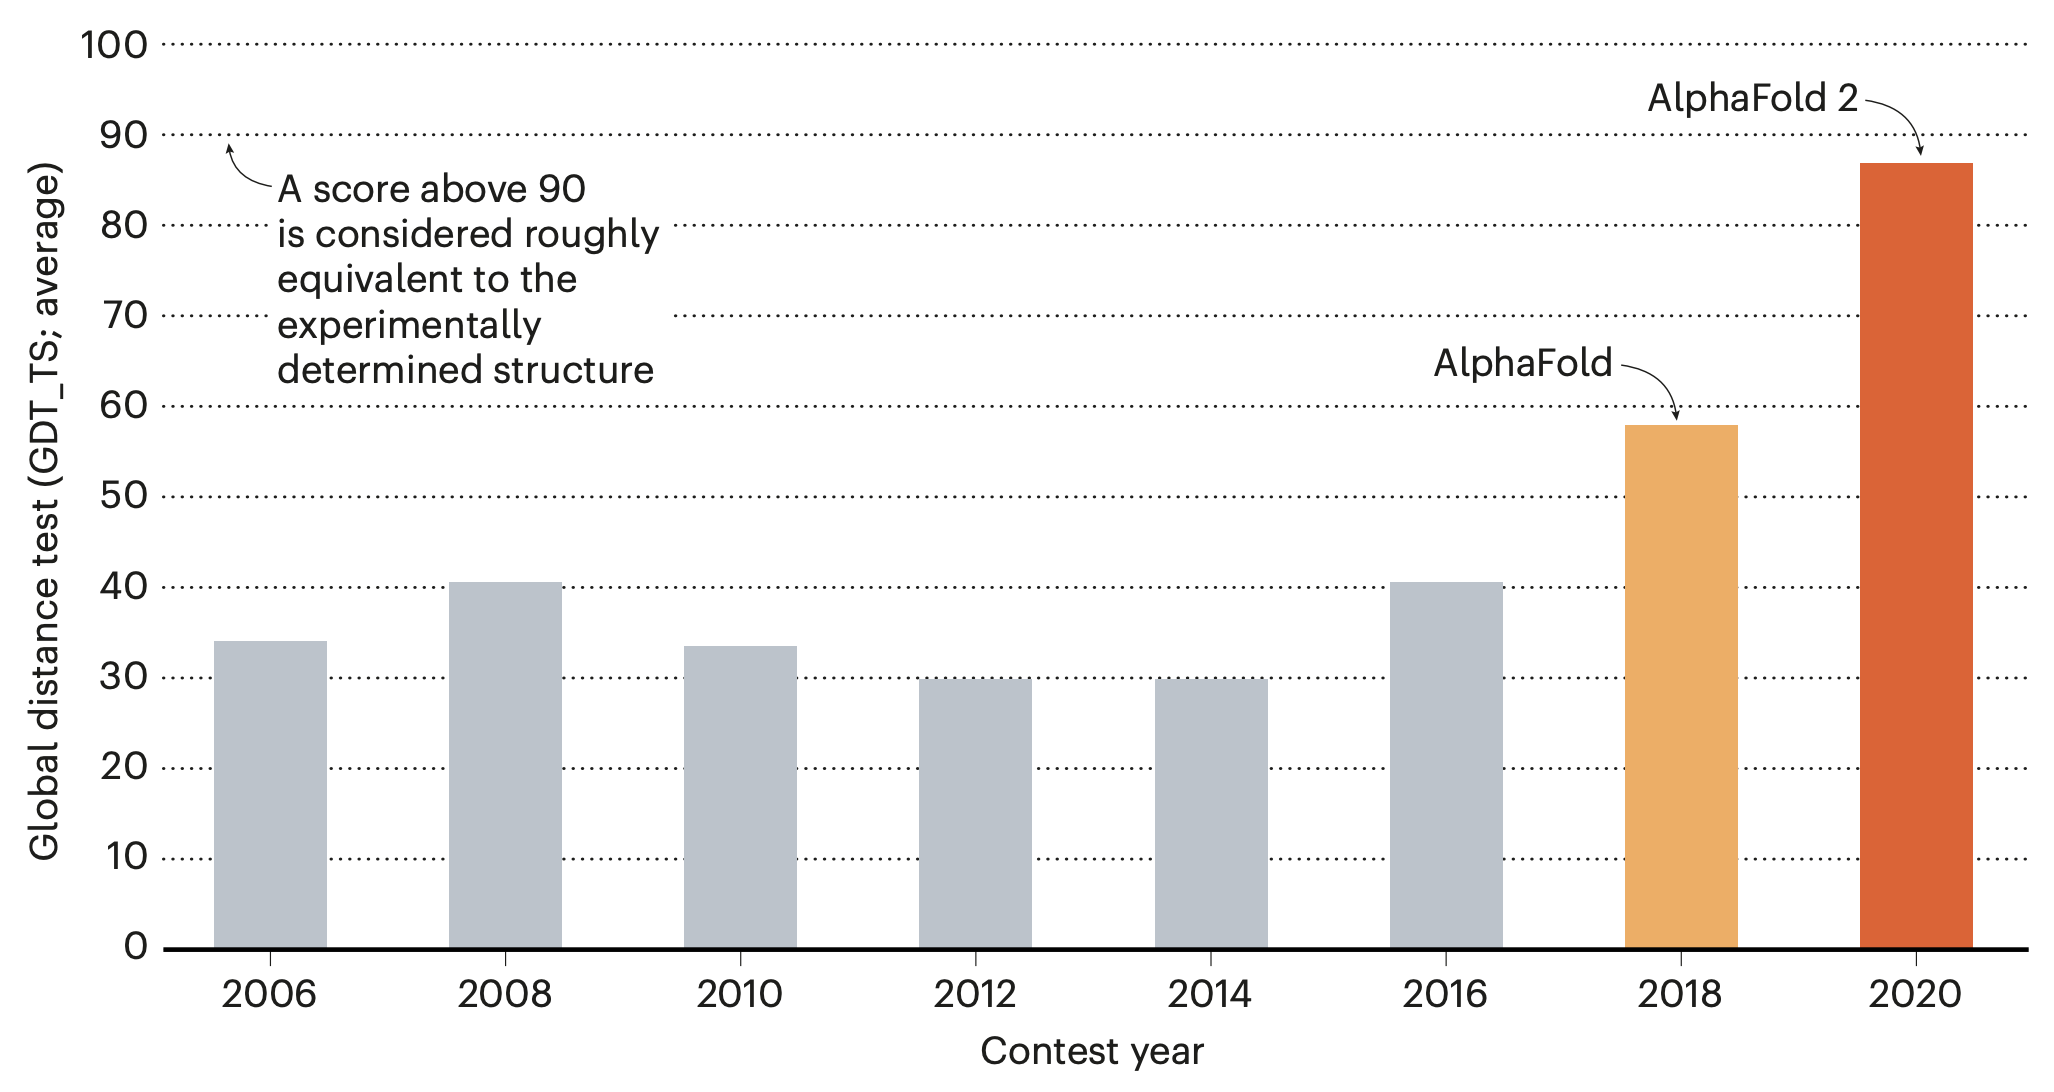
\includegraphics[width=0.9\columnwidth]{images/Deep_Mind.png}
  \caption{
      (\textit{Figura en inglés})
      $\textit{AlphaFold}$, las redes de $\textit{DeepMind}$, han revolucionado el campo de la predicción de la estructura 3D de las proteínas a partir de su secuencia lineal.
      Sus predicciones están cerca de tener un 90\% de similitud con los resultados experimentales.
      Fuente \cite{callawayItWillChange2020}
  }
  \label{fig:Deep_Mind}
\end{figure} 

 

